\documentclass[12pt]{article}
\usepackage[a4paper, total={6in, 10in}]{geometry}

\usepackage{graphicx}
\usepackage{abstract}
\usepackage{hyperref}
\usepackage{listings}
\usepackage{indentfirst}
\usepackage{amssymb}
\usepackage{titling}
\usepackage{mwe}
\usepackage{fancyhdr}
\usepackage{setspace}

\graphicspath{ {./images/} }
\renewcommand{\abstractname}{\small{\begin{center}Timestamps\end{center}\vspace{-4ex}}}

\setlength{\parskip}{3mm}   % Add space between paragraphs.
\setlength{\parindent}{0.5in}
\onehalfspacing
\setlength{\droptitle}{-35pt}

\fancypagestyle{plain}{
    \vspace{3ex}
    \fancyhead[L]{October 17th, 2020}
    \renewcommand{\headrulewidth}{0.5pt}
}

\pretitle{\begin{center} \LARGE \textbf}
\posttitle{\end{center} \vspace{-3ex}}
\preauthor{\begin{center} \large}
\postauthor{\end{center} \vspace{-3ex}}
\predate{\begin{center} \small \emph}
\postdate{\end{center} \vspace{-3ex}}

\title{Chapter \#3 Summary\\\Large+\\ Review Questions \#1-15}
\author{Chris Nutter\thanks{Dedicated to @QuesoGrande a.k.a. Jared D.}}
\date{CPSC 315}

% --> Here we go, satellite radio, y'all get hit with a...

\begin{document}
\maketitle

\begin{center} \vspace{-4ex}|\vspace{-3ex} \end{center}

\noindent\abstractname
\begin{center}
    \normalsize\textbf{10/08/2020 - 01:58:55 PM}\\
\end{center}
\normalsize

\tableofcontents    
\vspace{4ex}

% --> First Chapter

\section{Summary}
\indent The Internet being relatively new has changed the way we view humanity and the world as a whole. The Internet provides us with information in milliseconds which has helped countless people win arguments with people when they did not have the answer. The Internet is also the scariest invention since the Atomic Bomb as it has a huge potential to be the largest anti-privacy hotspot. Billion's of indexed pages allow for people to view information very quickly which is very useful because preserving facts is very important to maintaining a presence in society. The information is very easily manipulated however (especially on Wikipedia) which is easily edited to be stripped of "controversial information". Preserving information of all types is also something that is important as it prevents censorship in a world of progressive censorship being a problem. The book labels the Internet as "the best and worst of humanity" which is very, \emph{very} accurate; however, that can be labeled about most of the world in ways. The internet can be dark and twisted but also holds some of the greatest attributes of modern life. The worst of the Internet isn't even the "dark web", it's social media.\\
\indent Social media is becoming the biggest red flag of society as of lately. Facebook, Twitter, Linkedin all use your information and sell them for use in many activities that you may not was be apart of. Often times too it's people under the age of 18 which is \emph{really} scary. Social media in closed conditions however (IRC, Direct message through secure SSL encrypted lines) is still a viable option.\\
\indent Censorship is a very important novelty that is considered by many a human right. The Internet is the \#1 hotspot for preventing censorship. Anyone can create a website and make whatever they want for content and it'd be completely fine (assuming no illegal content is hosted). One problem with this is companies like Facebook who censor what you want to say on their platform that doesn't fit their narrative.\\
\indent While we get closer to a completely technological age, life is breaching a very important stage of what we should the Internet be capable of and the limits we set upon it. Whether it be watching videos or reading articles, the Internet is something that will not go away and that is not a bad thing; we, however, need to acknowledge its faults and learn to improve it over time.

\section{Questions}
    \begin{enumerate}
        \item Spam is very popular for a multitude of reasons. Sending an email in batch (around 100,000 emails) can only up to 10 minutes which is faster than sending physical mail. Someone can spend that time hoping to achieve a couple of innocent people's information, or whatever they plan on achieving, just by sending an email. 
        \item Spam is on the decline as people are finally starting to understand what spam looks like especially with spam filters. Google, despite being \emph{Google}, has created many magnificent algorithms including their spam filter. Their spam filter works 99\% of the time which is very impressive. Typically scams happen with advertisements on websites versus spam anymore.
        \item A good chunk of web browsing is done on mobile devices right now as it's quicker and easier to load a webpage on your phone on the go versus pulling out a laptop to look something up. My personal website is currently getting optimized for mobile layouts so it is very important to setup a mobile and base website layout. With apps, it's easier to view clean UI on an app versus just a plain webpage (especially) on mobile. People will take ease of capability nowadays so UI so becoming more important by the day.
        \item Texting is sent through radio towers while instant messaging is sent through the internet. Both have the ability to be encrypted which is good for the end users, but both have vulnerabilities. Instant messaging can still be tampered with by many people while texting is also a clean hotspot for spam messages.
        \item Facebook is a prime example of how social media has messed with news as they censor news outlets that do not fall under their agenda (typically conservative-based news outlets).
        \item The Internet is faster and easier than conventional newspapers. Pretty simple answer. However newspapers are still safer in a lot of ways being more of a public medium.
        \item Censorship is a person, company, outlet, etc. who silences a person for their point-of-view on topics whether that be physically silence or remove messages and anywhere in-between.
        \item The Internet is open to \emph{anybody}. Any human can buy a domain, host a server, and output whatever they want on the Internet. You cannot censor someone's website unless the government seizes your website for illegal content. News outlets, on the other hand, can cut off feed while you are talking.
        \item Broadcasters cannot say whatever they want because they are given a script to read from and if they deviate then they're finding a new job. Book publishers can make a story and send it out to anyone and that's out there for life.
        \item Sexting is very difficult to combat because with how encrypting is being done nowadays, lots people cannot tamper feeds as easily. At this point, it's up to the parents to teach their kids how to be responsible.
        \item The leading form of identity theft is probably done through social security. Your social security number is like a lock that is in your brain. If you give someone the lock, they will create duplicates and it's out there and you can never get a new one lock on your door.
        \item College students are fresh meat for identity theft because they are just starting life and they are able to use your information to affect the early stages of your employment.
        \item High-tech methods of identity theft:
            \begin{enumerate}
                \item Hacking into a bank account database.
                \item Creating a website that looks like you are selling a product but you are just stealing their credit card information.
            \end{enumerate}
            Low-tech methods of identity theft:
            \begin{enumerate}
                \item Robbing someone blindly.
                \item TeamViewer into someone's computer and pretending to be tech support.
            \end{enumerate}
        \item Cyberbullying is the concept of harassing an individual physically or mentally but using a technological product to aid.
        \item Technology releases dopamine similarly to pornography. Each click and sound you hear, your brain addresses and releases that dopamine which keeps you wanting to do it more and more. The more you do it the more your body gets inclined and hard to quick. It's very similar to nicotine or drugs.
     \end{enumerate}
        
\end{document} 

% Possibly Important LaTeX Functions %
% ================================== %

%   \begin{figure}[hbtp]
%       \centering
%       \fbox{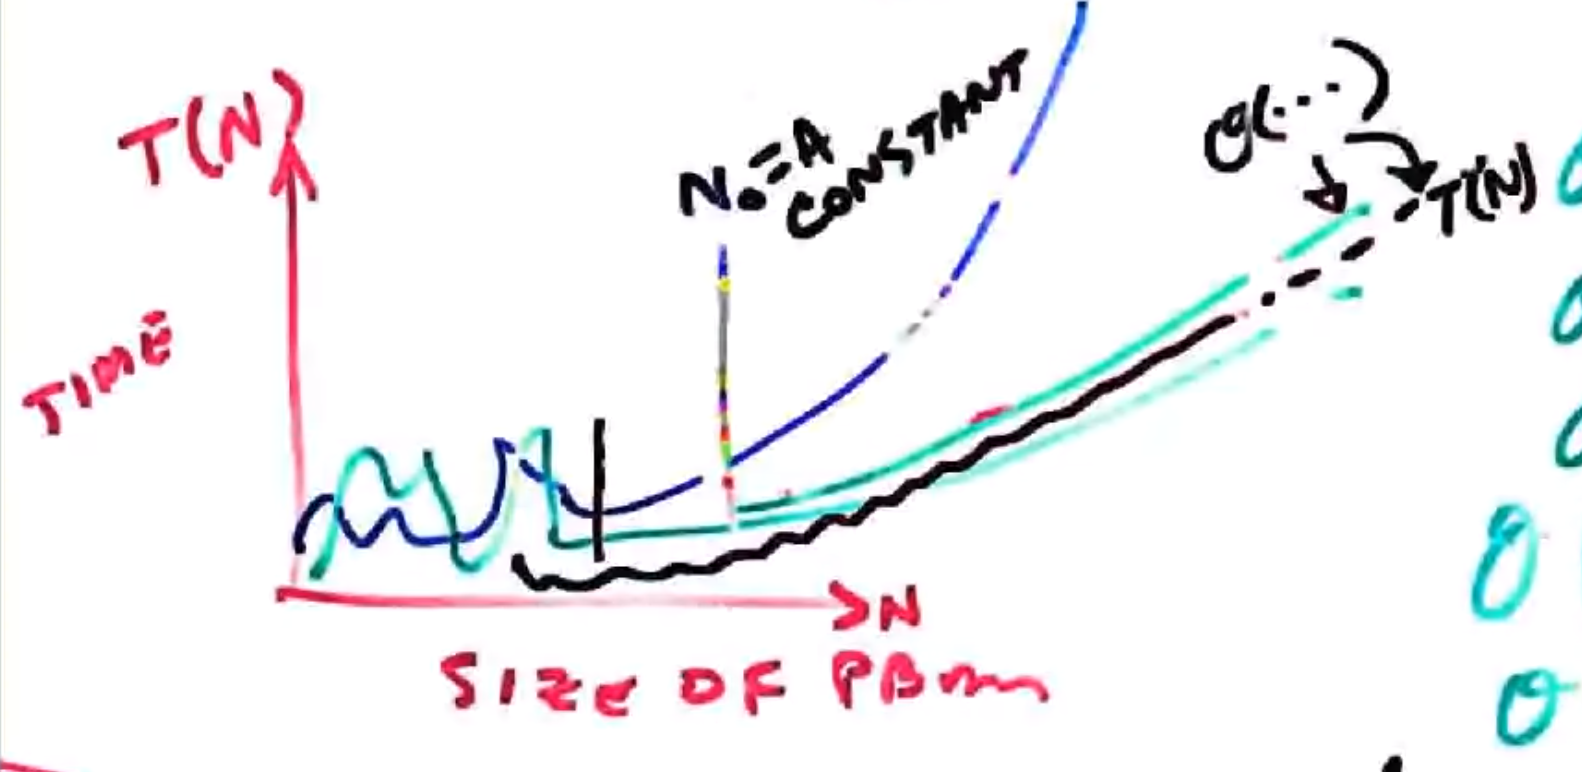
\includegraphics[width=13.8cm]{big_o.png}}
%       \caption{Big(O) Notation}
%   \end{figure}

%   \begin{lstlisting}[language=Python] 
%        print('hello world') 
%   \end{lstlisting}  

